%
%===============>>  ГРУППА 8-2 МОДУЛЬ 7  <<=============
%
\setmodule{7}

%BEGIN_FOLD % ====>>_____ Занятие 1 _____<<====
\begin{class}[number=1]
	\begin{definit}
		\textbf{Синусом} острого угла в прямоугольном треугольнике называется отношение противолежащего катета к гипотенузе.
	\end{definit}
	\begin{definit}
		\textbf{Косинусом} острого угла в прямоугольном треугольнике называется отношение прилежащего катета к гипотенузе.
	\end{definit}
	\begin{definit}
		\textbf{Тангенсом} острого угла в прямоугольном треугольнике называется отношение противолежащего катета к прилежащему катету.
	\end{definit}
	\begin{listofex}
		\item В треугольнике \( ABC \) угол \( C \) равен \( 90 \) градусов, \( AC=6 \), \( AB=20 \). Найдите \( \sin\angle B \).
		\item  В треугольнике \( ABC \) угол \( C \) равен \( 90 \) градусов, \( BC=9 \), \( AB=20 \). Найдите \( \cos\angle B \).
		\item В треугольнике \( ABC \) угол \( C \) равен \( 90 \) градусов, \( BC=9 \), \( AC=27 \). Найдите \( \tg\angle B \).
		\item Найдите синус, косинус и тангенс углов \( A \) и \( B \) треугольника \( ABC \) с прямым углом \( C \), если:
		\begin{tasks}(2)
			\task \( BC=8 \), \( AB=17 \)
			\task \( BC=21 \), \( AC=20 \)
			\task \( BC=1 \), \( AC=2 \)
		\end{tasks}
		\end{listofex}
		\begin{definit}
		\textbf{Основное тригонометрическое тождество:} \[\sin^2\alpha+\cos^2\alpha=1\]
		\end{definit}
		\begin{listofex}[resume]
		\item Докажите основное тригонометрическое тождество с помощью теоремы Пифагора.
		\item Найдите, зная, что угол острый:
		\begin{tasks}(1)
			\task \( \sin\alpha \) и \( \tg\alpha \), если \( \cos\alpha=\dfrac{1}{2} \)
			\task \( \cos\alpha \) и \( \tg\alpha \), если \( \sin\alpha=\dfrac{\sqrt{3}}{2} \)
		\end{tasks}
		\item В прямоугольном треугольнике один из катетов равен \( 10 \), а противолежащий угол равен \( 50\degree \). Выразите значение второго катета и гипотенузы через синус и тангенс известного угла.
		\item Катеты прямоугольного треугольника равны \( 12 \) и \( 15 \). Найдите гипотенузу и тангенсы острых углов. Во сколько раз тангенс одного угла больше другого? Возьмите за длины катетов значения \( a \) и \( b \). Каково отношение тангенсов в этом случае? Какой вывод можно сделать?
		\item Найдите углы ромба с диагоналями \( 2\sqrt{3} \) и \( 2 \).
		\item Стороны прямоугольника равны \( 3 \) см и \( \sqrt{3} \) см. Найти углы, которые образует диагональ со стороной прямоугольника.
		\item В треугольнике \( ABC \) угол \( C \) равен \( 90\degree \), \( \sin A=\dfrac{4}{5} \), \( AC=9 \). Найдите \( AB \).
		\end{listofex}
\end{class}
%END_FOLD

%BEGIN_FOLD % ====>>_____ Занятие 2 _____<<====
\begin{class}[number=2]
	\begin{listofex}
		\item Катеты прямоугольного треугольника равны \( \sqrt{15} \) и \( 1 \). Найдите синус наименьшего угла этого треугольника.
		\item В треугольнике \( ABC \) угол \( C \) равен \( 90\degree \), \( AC=12 \), \( \tg A=\dfrac{2\sqrt{10}}{3} \).  Найдите \( AB \).
		\item В треугольнике \( ABC \) угол \( C \) равен \( 90\degree \), \( \sin A=\dfrac{4}{5} \), \( AC=9 \). Найдите \( AB \).
		\item Найдите синус меньшего острого угла между	диагональю прямоугольника и его стороной, если периметр прямоугольника равен \( 34 \) см, а одна из сторон --- \( 12 \) см. 
		\item Тангенс острого угла прямоугольного треугольника равен \( \dfrac{2}{5} \), а один из катетов на \( 6 \) см больше другого. Найдите площадь треугольника. 
		\item Площадь прямоугольного треугольника равна \( 32\sqrt{3} \). Один из острых углов равен \( 30\degree \). Найдите длину гипотенузы.
		\item Основание равнобедренного треугольника равно \( 8 \) см, тангенс угла при основании равен \( 2 \). Найдите площадь треугольника. 
		\item Периметр равнобедренного треугольника равен \( 64 \) см, косинус угла при основании равен \( 0,6 \). Найдите площадь треугольника.
		\item Найдите, зная, что угол \( \alpha \) острый:
		\begin{tasks}(1)
			\task \( \sin\alpha, \cos\alpha \), \quad если \( \tg\alpha=\dfrac{3}{4} \)
			\task \( \tg \alpha \),\quad если \( \sin \alpha=\dfrac{5}{13} \)
		\end{tasks}
	\end{listofex}
\end{class}
%END_FOLD

%BEGIN_FOLD % ====>>_ Домашняя работа 1 _<<====
\begin{homework}[number=1]
	\begin{listofex}
		\item В треугольнике \( ABC \) угол \( C \) равен \( 90\degree \), \( AC=9 \), \( AB=25 \). Найдите \( \sin B \).
		\item В треугольнике \( ABC \) угол \( C \) равен \( 90\degree \), BC\( =4 \), \( AC=28 \). Найдите \( \tg B \).
		\item В треугольнике \( ABC \) угол \( C \) равен \( 90\degree \), \( \sin B=\dfrac{5}{17} \), \( AB=51 \). Найдите \( AC \).
		\item В треугольнике\( ABC \) угол \( C \) равен \( 90\degree \), \( \tg B=\dfrac{8}{5} \), \( BC=20 \). Найдите \( AC \).
		\item Синус острого угла \( A \) треугольника \( ABC \) равен \( \dfrac{2\sqrt{6}}{5} \). Найдите \( \cos A \).
		\item В равнобедренном треугольнике \( ABC \) \( AB=BC \). Угол \( B \) равен \( 120\degree \), а высота, опущенная на основание равна \( \dfrac{\sqrt{3}}{2} \). Найдите площадь треугольника.
	\end{listofex}
\end{homework}
%END_FOLD

%BEGIN_FOLD % ====>>_____ Занятие 3 _____<<====
\begin{class}[number=3]
	\begin{definit}
		\textbf{Первый признак подобия треугольников:} два угла одного треугольника соответственно равны двум углам другого.
	\end{definit}
	\begin{definit}
		\textbf{Второй признак подобия треугольников:} две стороны одного треугольника пропорциональны двум сторонам другого, и углы, образованные этими сторонами, равны.
	\end{definit}
	\begin{definit}
		\textbf{Третий признак подобия треугольников:} три стороны одного треугольника пропорциональны трём сторонам другого.
	\end{definit}
	\begin{listofex}
		\item Подобны ли треугольники \( ABC \) и \( A_1B_1C_1\), если известно, что:
		\begin{tasks}(1)
		\task \(AB=10\) см; \(BC=5\) см; \( AC=7 \) см; \( A_1B_1=15\) см; \( B_1C_1=7,5\) см; \(A_1C_1=9,5\) см?
		\task \( \angle A=37\degree \), \( \angle B=48\degree\), \( \angle C_1=95\degree \), \( \angle B_1= 48\degree \)?
		\task \( AB=10 \) см, \(BC=8\) см, \(A_1B_1=5\) см, \(A_1C_1=3\) см, \(\angle C=\angle C_1=90\degree\)?
	\end{tasks}
		\item Человек двухметрового роста измерил свою тень от уличного фонаря. Она оказалась равной \( 1 \) метру. Потом он измерил расстояние до фонаря --- оно оказалось равно \( 4 \) метра. Какова высота фонаря?
		\item Из треугольника вырезали ромб так, как показано на рисунке. Найдите сторону ромба, если боковые стороны треугольника равны \( 3 \) и \( 6 \).
		\begin{center}
			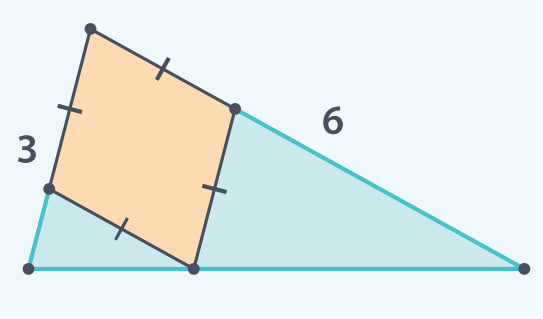
\includegraphics[align=t, width=0.3\linewidth]{\picpath/G82M7L3}
		\end{center}
		\item Фотографию, размеры которой \( 10 X 15 \) см, заключили в рамку подобной формы, ширина которой по горизонтали равна \( 3 \) см. Найдите высоту рамки по вертикали.
		\item Ширина большого пальца взрослого мужчины в среднем равна одному дюйму или
		\( 2,5 \) см, а расстояние от глаза до этого пальца на вытянутой руке --- примерно \( 60 \) см. Человек	увидел в небе самолёт, вытянул руку и закрыл его большим пальцем. На каком расстоянии
		от человека находится самолёт, если длина его фюзеляжа обычно около \( 75 \) м?
		\item Диаметр Луны приблизительно \( 3400 \) км, а от Земли она находится на расстоянии	\( 408000 \) км. Какого диаметра нужно изготовить светящийся белый шар на сцене Большого театра, чтобы зрителям из середины зала он казался такой же величины, как и луна на небе? Среднее расстояние от середины зала до задника сцены в нём равно \( 33 \) м.
		\item Основание равнобедренного треугольника равно \( 3 \), а его боковые стороны равны \( 7 \). На боковых сторонах взяли по одной точке так, что три отмеченных на рисунке отрезка равны. Найдите длину этих отрезков.
		\begin{center}
			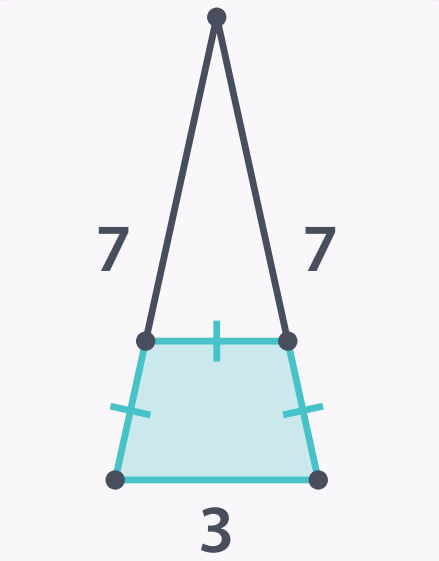
\includegraphics[align=t, width=0.3\linewidth]{\picpath/G82M7L3-2}
		\end{center}
		\item Основания трапеции равны \( 3 \) и \( 8 \). Отрезок с концами на её боковых сторонах параллелен основаниям и имеет длину \( 6 \). В каком отношении его концы делят боковые стороны трапеции?
		\item Отрезок с концами на боковых сторонах	трапеции параллелен её основаниям \( 5 \) и \( 8 \). Найдите его длину, если он делится диагоналями трапеции на три равные части. Сколько решений у задачи?
	\end{listofex}
\end{class}
%END_FOLD

%BEGIN_FOLD % ====>>_____ Занятие 4 _____<<====
\begin{class}[number=4]
	\begin{listofex}
		\item Подобны ли равнобедренные треугольники, если они имеют:
		\begin{tasks}(1)
			\task по равному острому углу;
			\task по равному тупому углу;
			\task по прямому углу?			
		\end{tasks}
		\item На стороне \( CD \) параллелограмма \( ABCD \) отмечена точка \( E \). Прямые \( AE \) и \( BC \) пересекаются в точке \( F \). Найдите: 
		\begin{tasks}(1)
			\task \( EF \) и \( FC \), если \( DE=8 \) см, \( EC=4 \) см, \( BC=7 \) см, \( AE=10 \) см;
			\task \( DE \) и \( EC \), если \( AB=8 \) см, \( AD=5 \) см, \( CF=2 \) см.
		\end{tasks}  
		\item Диагонали параллелограмма \( ABCD \) пересекаются в точке \( O \). Точки \( F \) и \( T \) лежат соответственно на отрезках \( OC \) и \( OD \) так, что \( CF:FO=1:3 \) и \( DT:TO=1:3 \). Докажите, что треугольники \( AOB \) и \( FOT \) подобны.
		\item Точки \( O \) и \( F \) лежат соответственно на сторонах \( AB \) и \( BC \) треугольника \( ABC \). Докажите, что прямые \( FO \) и \( AC \) параллельны, если \( AB=48 \) см, \( CB=32 \) см, \( AO=18 \) см, \( BF=20 \) см.
		\item Человек ростом \( 2 \) метра, отойдя от телеграфного столба на \( 10 \) метров, заметил, что этот столб «закрыл» верхушку дерева. Найдите высоту дерева, если высота столба равна \( 8 \) м, а расстояние от столба до дерева равно \( 35 \) м?
		\item Из прямоугольного треугольника с катетами \( 6 \) и \( 7 \) вырезали прямоугольник так, как это показано на рисунке. Найдите периметр этого прямоугольника, если одна его сторона в два раза больше другой.
		\begin{center}
			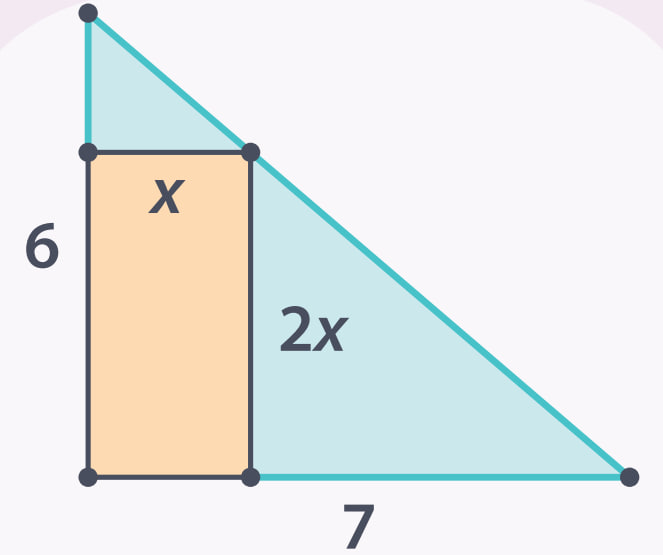
\includegraphics[align=t, width=0.3\linewidth]{\picpath/G82M7L4}
		\end{center}
		\item Докажите, что отношение периметров подобных треугольников равно коэффициенту подобия.
		\item Докажите, что высота прямоугольного треугольника, проведённая из вершины прямого угла, делит треугольник на два подобных треугольника
	\end{listofex}
\end{class}
%END_FOLD

%BEGIN_FOLD % ====>>_ Домашняя работа 2 _<<====
\begin{homework}[number=2]
	\begin{listofex}
		\item Тень от вершины пирамиды Хеопса легла	в \( 70 \) шагах от её подножия и оказалась	одинаково удалена от двух её углов. В то же самое время недалеко от пирамиды человек воткнул в песок свой посох и	заметил, что тень от него была на треть	больше высоты посоха. Определите по	этим данным высоту пирамиды, если она имеет квадратное основание со стороной, равной \( 230 \) шагам.
		\item Предком фотоаппарата по праву считается старинная камера-обскура или «темная комната». Она представляет собой черный ящик, в стенке которого проделано маленькое отверстие. В яркий солнечный
		день на противоположной стенке такого ящика можно видеть перевёрнутые и	уменьшенные изображения предметов, находящихся вне этого ящика. Определите по данным на рисунке высоту дерева, если его изображение на экране камеры обскуры имеет длину \( 15 \) см.
		\begin{center}
			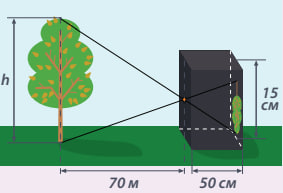
\includegraphics[align=t, width=0.3\linewidth]{\picpath/G82M7H2}
		\end{center}
		\item На стороне \( AC \) треугольника \( ABC \) отложен отрезок \( AM \), равный третьей части стороны \( AB \), а на стороне \( AB \) --- отрезок \( AN \), равный третьей части стороны \( AC \). Найдите \( MN \), если \( BC=15 \).
	\end{listofex}
\end{homework}
%END_FOLD

%BEGIN_FOLD % ====>>_____ Занятие 5 _____<<====
\begin{class}[number=5]
	\begin{listofex}
		\item Решите системы неравенств:
		\begin{tasks}(2)
			\task \( \left\{
			\begin{array}{l}
				x-7,4\ge0,\\
				x+2\ge3
			\end{array}
			\right. \)
			\task \( \left\{
			\begin{array}{l}
				-12+3x<0,\\
				9-4x>-23
			\end{array}
			\right. \)
		\end{tasks}
		\item Каждая из сторон \( AB \) и \( AC \) треугольника \( ABC \) разделена соответственно точками \( M \) и \( N \) в отношении \( 2:3 \), считая	от точки \( A \). Докажите, что \( MN || BC \), и найдите \( MN \), если \( BC=20 \).
		\item Точка \( M \) лежит на боковой стороне \( AB \) трапеции \( ABCD \), причем \( AM:MB=1:2 \). Прямая, проходящая через точку \( M \) параллельно основаниям \( AD \) и \( BC \), пересекает
		боковую сторону \( CD \) в точке \( N \). Найдите \( MN \), если \( AD=a \)	и \( BC=b \).
		\item Точка \( M \) лежит на боковой стороне \( AC \) равнобедренного треугольника \( ABC \) с основанием \( BC \), причем \( BM=BC \). Найдите \( MC \), если \( BC=1 \) и \( AB=2 \).
		\item Прямоугольный треугольник с катетами, равными \( 6 \)	и \( 8 \), вписан квадрат, имеющий с треугольником общий прямой угол. Найдите сторону квадрата.
		\item Докажите, что медиана \( AM \) треугольника \( ABC \) делит пополам любой отрезок с концами на \( AB \) и \( AC \), параллельный стороне \( BC \).
		\item Существует ли на окружности, заданной уравнением \( (x-3)^2+(y+1)^2=7 \) точка с абциссой, равной \( 1,5 \)? с ординатой, равной \( -4,9 \)?
		\end{listofex}
\end{class}
%END_FOLD

%BEGIN_FOLD % ====>>_____ Занятие 6 _____<<====
\begin{class}[number=6]
	\begin{listofex}
		\item \exercise{2596}
		\item \exercise{2598}
		\item \exercise{2601}
		\item \exercise{2602}
		\item \exercise{2605}
		\item \exercise{2612}
		\item \exercise{2613}
	\end{listofex}
\end{class}
%END_FOLD

%BEGIN_FOLD % ====>>_ Домашняя работа 3 _<<====
\begin{homework}[number=3]
	\begin{listofex}
		\item \exercise{2597}
		\item \exercise{2599}
		\item \exercise{2604}
	\end{listofex}
\end{homework}
%END_FOLD

%BEGIN_FOLD % ====>>_____ Занятие 7 _____<<====
\begin{class}[number=7]
	\title{Подготовка к проверочной}
	\begin{listofex}
		\item Занятие 7
	\end{listofex}
\end{class}
%END_FOLD

=%BEGIN_FOLD % ====>>_ Проверочная работа _<<====
\begin{exam}
	\begin{listofex}
		\item Проверочная
	\end{listofex}
\end{exam}
%END_FOLD